\documentclass{standalone}
\usepackage{tikz}
\begin{document}
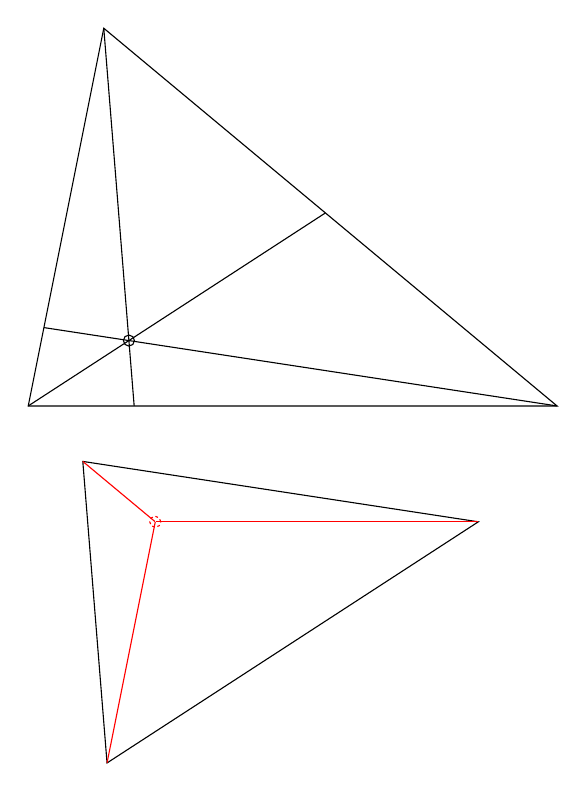
\begin{tikzpicture}[x=1pt,y=1pt]
\draw (50.39,-16.96) -- (61.37,-153.45);
\draw (23.09,-153.45) -- (130.48,-83.70);
\draw (214.18,-153.45) -- (28.75,-125.13);
\draw (59.47,-129.82) circle (2.00);
\draw (23.09,-153.45) -- (214.18,-153.45) -- (50.39,-16.96) -- cycle;
\draw (42.81,-173.49) -- (51.57,-282.45) -- (185.74,-195.31) -- cycle;
\draw[red] (68.90,-195.23) -- (42.81,-173.49);
\draw[red] (69.14,-195.31) -- (185.73,-195.31);
\draw[red] (68.98,-195.41) -- (51.57,-282.45);
\draw[red, dash pattern=on 1pt] (69.00,-195.31) circle (2.00);
\end{tikzpicture}
\end{document}
